\documentclass[aspectratio=169]{beamer}
\usepackage[utf8]{inputenc}
\usepackage[T1]{fontenc}
\usepackage[magyar]{babel}
\usepackage{hyperref}
\usepackage{biblatex}
\usepackage{csquotes}
\usepackage{graphicx}

% Acous-optics Bragg Diffraction Interaction of sound and light
% Doppler-shift Acousto optic devices

\setbeamertemplate{navigation symbols}{}
%\setbeamertemplate{footline}[frame number]
\setbeamertemplate{caption}{\insertcaption}

\usetheme{Madrid}
\usecolortheme{default}
\renewcommand{\figurename}{}
\newcommand{\framet}{\frametitle{\secname{} - \subsecname}}

\begin{document}
\title{Akusztooptika}
\subtitle{Bragg-diffrakció, fény és hang interakció,\\Doppler-effektus, akusztooptikai berendezések}
\author{Készítette: Illés Gergő}
\date{2023. május 02.}
\begin{frame}
\maketitle
\end{frame}

\begin{frame}
\frametitle{Tartalomjegyzék}

\begin{columns}
\column{.90\textwidth}
\tableofcontents
\end{columns}
\end{frame}

\section{Bragg-diffrakció}
\begin{frame}
\frametitle{\secname}
\begin{columns}
\column{.6\textwidth}
\begin{itemize}
\item A röntgensugarak kristályokban történő diffrakcióját 1913-ban publikálták.
\item A jelenséget William Henry Bragg és fia William Lawrence Bragg fedezte fel és később róluk nevezték el.
\item A diffrakciót a rácsok egyes fősíkjairól visszaverődő sugarak interferenciája okozza.
\item Bragg-diffrakcióról beszélünk az akusztooptika témakörében is, de ilyenkor a diffrakció más okból jön létre
\end{itemize}
\column{.4\textwidth}
\begin{figure}
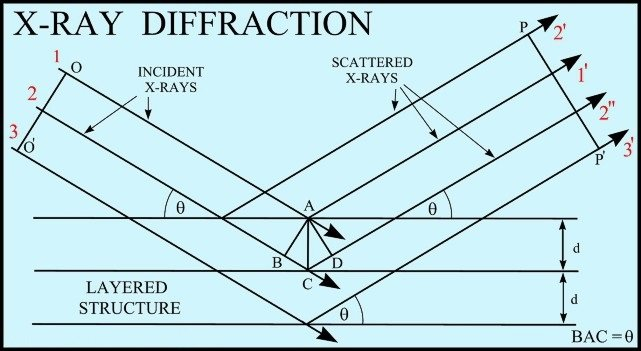
\includegraphics[width=.9\textwidth]{xrd6.jpg}
\caption{A Bragg diffrakció illusztrációja}
\end{figure}
\end{columns}
\end{frame}

\section{Fény és hang interakció}
\begin{frame}
\frametitle{\secname}
\begin{columns}
\column{.5\textwidth}
\begin{itemize}
\item Az akusztooptikában a kristály rácsperiódusánál jóval nagyobb hullámhosszakat használnak.
\item Ezen források általában lézerek a látható-, vagy ahhoz közeli tartományban sugároznak.
\item $n\lambda=2d\sin(\theta)$ - Röntgen diffrakció
\item $\lambda=2n\Lambda\sin(\alpha)$ - Akusztooptikai diffrakció
\end{itemize}
\column{.5\textwidth}
\begin{figure}
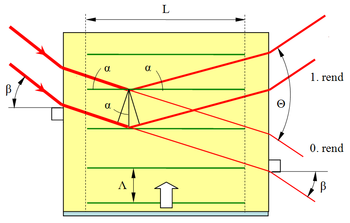
\includegraphics[width=.95\textwidth]{bragg-diff.png}
\caption{Akusztooptikai Bragg diffrakció}
\end{figure}
\end{columns}
\end{frame}

\begin{frame}
\begin{figure}
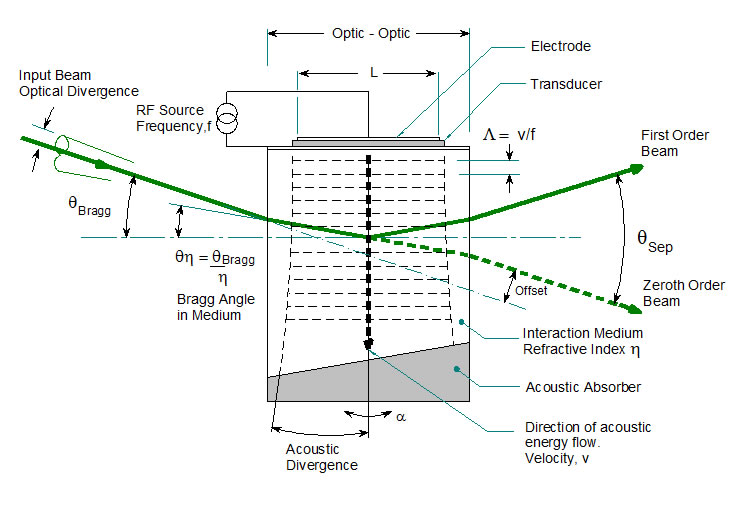
\includegraphics[width=.8\textwidth]{isomet.jpg}
\end{figure}
\end{frame}

\section{Hivatkozások}
\begin{frame}
\frametitle{\secname}
\begin{thebibliography}{99}
\footnotesize
\bibitem{physopen} \url{https://physicsopenlab.org/2018/01/18/bragg-diffraction/}
\bibitem{fizpedia} \url{https://fizipedia.bme.hu/index.php/Akusztooptikai_f\%C3\%A9nydiffrakci\%C3\%B3_vizsg\%C3\%A1lata}
\bibitem{isomet} \url{https://isomet.com/acousto_optics.html}
\end{thebibliography}
\end{frame}
\end{document}